\subsection{Mission Overview}

The CoderDojo Space Robotics project team will execute the mission by designing and constructing a CanSat that will be deployed manually. During the CanSat's descent, it must maintain a speed between 5 and 10 meters per second, while it simultaneously collects and transmits key environmental data. This data will include temperature, pressure, spatial positioning, and UV radiation levels. In addition to these, the CanSat is uniquely equipped to detect muons. All of this data will be transmitted in real-time to the ground station and stored onboard. After landing, the CanSat will signal its coordinates using a buzzer, activating the recovery system.

These key elements will play an essential role in accomplishing the mission objectives. Here is a brief explanation of each element:
\begin{itemize}[leftmargin=1.27cm, itemindent=0cm, topsep=2pt, label=\faTasks]
    \item[\faThermometerQuarter] \textbf{Sensor System}: A sensor system is critical to the mission's success as it helps to measure various parameters that are important for the experiment. The sensor system can measure parameters such as temperature, pressure, inertial performance, UV, and light intensity. These measurements will provide valuable data for the post-launch data analysis.
    \coloredbox{LightCyan1!50}{DeepSkyBlue4}{DeepSkyBlue4}{
        {During the descent, the CanSat will record, store, and transmit the following data:
        \begin{multicols}{2}[\vspace{-0.6\baselineskip}]
            \begin{itemize}[noitemsep, topsep=0pt, label=\ding{111}]
                \item Humidity and air temperature
                \item Barometric pressure
                \item GPS Location
                \item Magnetic field
                \item Orientation
                \item Position in space using a gyroscope
                \item UV Index
            \end{itemize}
        \end{multicols}
        \vspace*{-0.75\baselineskip}
        }
    }
    \item[\faMicrochip] \textbf{Microcontroller}: The microcontroller is responsible for controlling the various subsystems of the CanSat. It provides a reliable and efficient way to control the CanSat's functions, making it a crucial part of the overall system.
    \item[\faBroadcastTower] \textbf{Telemetry Syste}m: The telemetry system is responsible for sending data back to the ground station. It uses GSM and RF modules to transmit data, which can be analyzed in real time by the mission team. This system helps to ensure that the mission objectives are met and that the data collected is of high quality.
    \item[ \faParachuteBox] \textbf{Recovery System}: The recovery system is essential to ensure the CanSat is safely returned to the ground. It consists of audible alarms that alert the ground station to the CanSat's location. This system will help to prevent damage to the CanSat and ensure that the data collected during the mission is preserved.
    \item[\faChartBar] \textbf{Post-Launch Data Analysis}: Post-launch data analysis is essential for interpreting the data collected during the mission. It allows the mission team to evaluate the success of the mission and determine whether the mission objectives were met. This analysis can help to inform future missions and experiments. 
\end{itemize}

%\begin{figure}[htbp]
%  \centering
%  \includesvg{img_Block_Diagram_2023.svg}
%  \caption{svg image}
%\end{figure}

\begin{figure}[htbp]
\centering
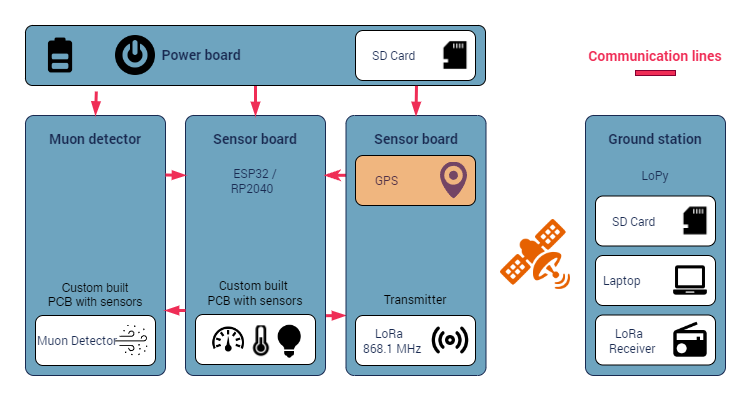
\includegraphics[width=0.9\linewidth]{RCRC_2024Block.drawio.png}
\caption{\small{Base block diagram for the CanSat and the ground station.}}
\label{fig:bloc_diagrame}
\end{figure}

Several onboard devices will make the mission possible, the key ones being:
    \begin{multicols}{2}[\vspace{-0.5\baselineskip}]
        \begin{itemize}[leftmargin=1.75cm,itemindent=0cm, noitemsep, topsep=2pt, label=\faCheck]
            \item[\faMicrochip] MicroController (ESP32 Wroom or Raspberry Py PR2040)
            % \item[\faCamera] Cameras (ESP32 With Camera Module OV2640)
            \item[ \faWifi] Data transceiver (LoRa)
            \item[\faThermometerQuarter] Humidity and temperature sensors %(BME 688, MCP 9808)
            \item[\faMapMarked] GPS (L76GNSS)
            \item[\faCompass] Navigation sensor %(LSM6DS33 gyroscope \& LIS3MDL compass )
            \item[\faBatteryHalf] High-performance batteries
            \item[\faRadiation] SiPM (Silicon photomultiplier) detector for muons
            \item[\newaltitudeicon] Altimeter %(LPS25H)
            % \item[\newgsmicon] GSM module (SIM800L)
        \end{itemize}
        \vspace*{-0.75\baselineskip}
    \end{multicols}

% \sout{The ESP32 and Arduino Nano 33 BLE Sense boards are designed to collect data from various sensors during the flight, including location, temperature, and pressure. This data is stored on an SD card for later analysis, but it is also transmitted to the base station in real-time using the LoRa protocol.

% In addition to collecting data from sensors, the boards also receive data from two GPS modules. This data is routed to the GSM communication module, which sends the GPS coordinates of the CanSat to the base station. This allows the mission team to track the CanSat's location and monitor its progress during the flight.

% Overall, the combination of the ESP32 and Arduino Nano 33 BLE Sense boards provides a reliable and efficient way to collect and transmit data during the CanSat's flight. The data collected can be analyzed after the mission to gain insights into various environmental factors and improve future missions.}

